\documentclass[1p]{elsarticle_modified}
%\bibliographystyle{elsarticle-num}

%\usepackage[colorlinks]{hyperref}
%\usepackage{abbrmath_seonhwa} %\Abb, \Ascr, \Acal ,\Abf, \Afrak
\usepackage{amsfonts}
\usepackage{amssymb}
\usepackage{amsmath}
\usepackage{amsthm}
\usepackage{scalefnt}
\usepackage{amsbsy}
\usepackage{kotex}
\usepackage{caption}
\usepackage{subfig}
\usepackage{color}
\usepackage{graphicx}
\usepackage{xcolor} %% white, black, red, green, blue, cyan, magenta, yellow
\usepackage{float}
\usepackage{setspace}
\usepackage{hyperref}

\usepackage{tikz}
\usetikzlibrary{arrows}

\usepackage{multirow}
\usepackage{array} % fixed length table
\usepackage{hhline}

%%%%%%%%%%%%%%%%%%%%%
\makeatletter
\renewcommand*\env@matrix[1][\arraystretch]{%
	\edef\arraystretch{#1}%
	\hskip -\arraycolsep
	\let\@ifnextchar\new@ifnextchar
	\array{*\c@MaxMatrixCols c}}
\makeatother %https://tex.stackexchange.com/questions/14071/how-can-i-increase-the-line-spacing-in-a-matrix
%%%%%%%%%%%%%%%

\usepackage[normalem]{ulem}

\newcommand{\msout}[1]{\ifmmode\text{\sout{\ensuremath{#1}}}\else\sout{#1}\fi}
%SOURCE: \msout is \stkout macro in https://tex.stackexchange.com/questions/20609/strikeout-in-math-mode

\newcommand{\cancel}[1]{
	\ifmmode
	{\color{red}\msout{#1}}
	\else
	{\color{red}\sout{#1}}
	\fi
}

\newcommand{\add}[1]{
	{\color{blue}\uwave{#1}}
}

\newcommand{\replace}[2]{
	\ifmmode
	{\color{red}\msout{#1}}{\color{blue}\uwave{#2}}
	\else
	{\color{red}\sout{#1}}{\color{blue}\uwave{#2}}
	\fi
}

\newcommand{\Sol}{\mathcal{S}} %segment
\newcommand{\D}{D} %diagram
\newcommand{\A}{\mathcal{A}} %arc


%%%%%%%%%%%%%%%%%%%%%%%%%%%%%5 test

\def\sl{\operatorname{\textup{SL}}(2,\Cbb)}
\def\psl{\operatorname{\textup{PSL}}(2,\Cbb)}
\def\quan{\mkern 1mu \triangleright \mkern 1mu}

\theoremstyle{definition}
\newtheorem{thm}{Theorem}[section]
\newtheorem{prop}[thm]{Proposition}
\newtheorem{lem}[thm]{Lemma}
\newtheorem{ques}[thm]{Question}
\newtheorem{cor}[thm]{Corollary}
\newtheorem{defn}[thm]{Definition}
\newtheorem{exam}[thm]{Example}
\newtheorem{rmk}[thm]{Remark}
\newtheorem{alg}[thm]{Algorithm}

\newcommand{\I}{\sqrt{-1}}
\begin{document}

%\begin{frontmatter}
%
%\title{Boundary parabolic representations of knots up to 8 crossings}
%
%%% Group authors per affiliation:
%\author{Yunhi Cho} 
%\address{Department of Mathematics, University of Seoul, Seoul, Korea}
%\ead{yhcho@uos.ac.kr}
%
%
%\author{Seonhwa Kim} %\fnref{s_kim}}
%\address{Center for Geometry and Physics, Institute for Basic Science, Pohang, 37673, Korea}
%\ead{ryeona17@ibs.re.kr}
%
%\author{Hyuk Kim}
%\address{Department of Mathematical Sciences, Seoul National University, Seoul 08826, Korea}
%\ead{hyukkim@snu.ac.kr}
%
%\author{Seokbeom Yoon}
%\address{Department of Mathematical Sciences, Seoul National University, Seoul, 08826,  Korea}
%\ead{sbyoon15@snu.ac.kr}
%
%\begin{abstract}
%We find all boundary parabolic representation of knots up to 8 crossings.
%
%\end{abstract}
%\begin{keyword}
%    \MSC[2010] 57M25 
%\end{keyword}
%
%\end{frontmatter}

%\linenumbers
%\tableofcontents
%
\newcommand\colored[1]{\textcolor{white}{\rule[-0.35ex]{0.8em}{1.4ex}}\kern-0.8em\color{red} #1}%
%\newcommand\colored[1]{\textcolor{white}{ #1}\kern-2.17ex	\textcolor{white}{ #1}\kern-1.81ex	\textcolor{white}{ #1}\kern-2.15ex\color{red}#1	}

{\Large $\underline{12a_{1203}~(K12a_{1203})}$}

\setlength{\tabcolsep}{10pt}
\renewcommand{\arraystretch}{1.6}
\vspace{1cm}\begin{tabular}{m{100pt}>{\centering\arraybackslash}m{274pt}}
\multirow{5}{120pt}{
	\centering
	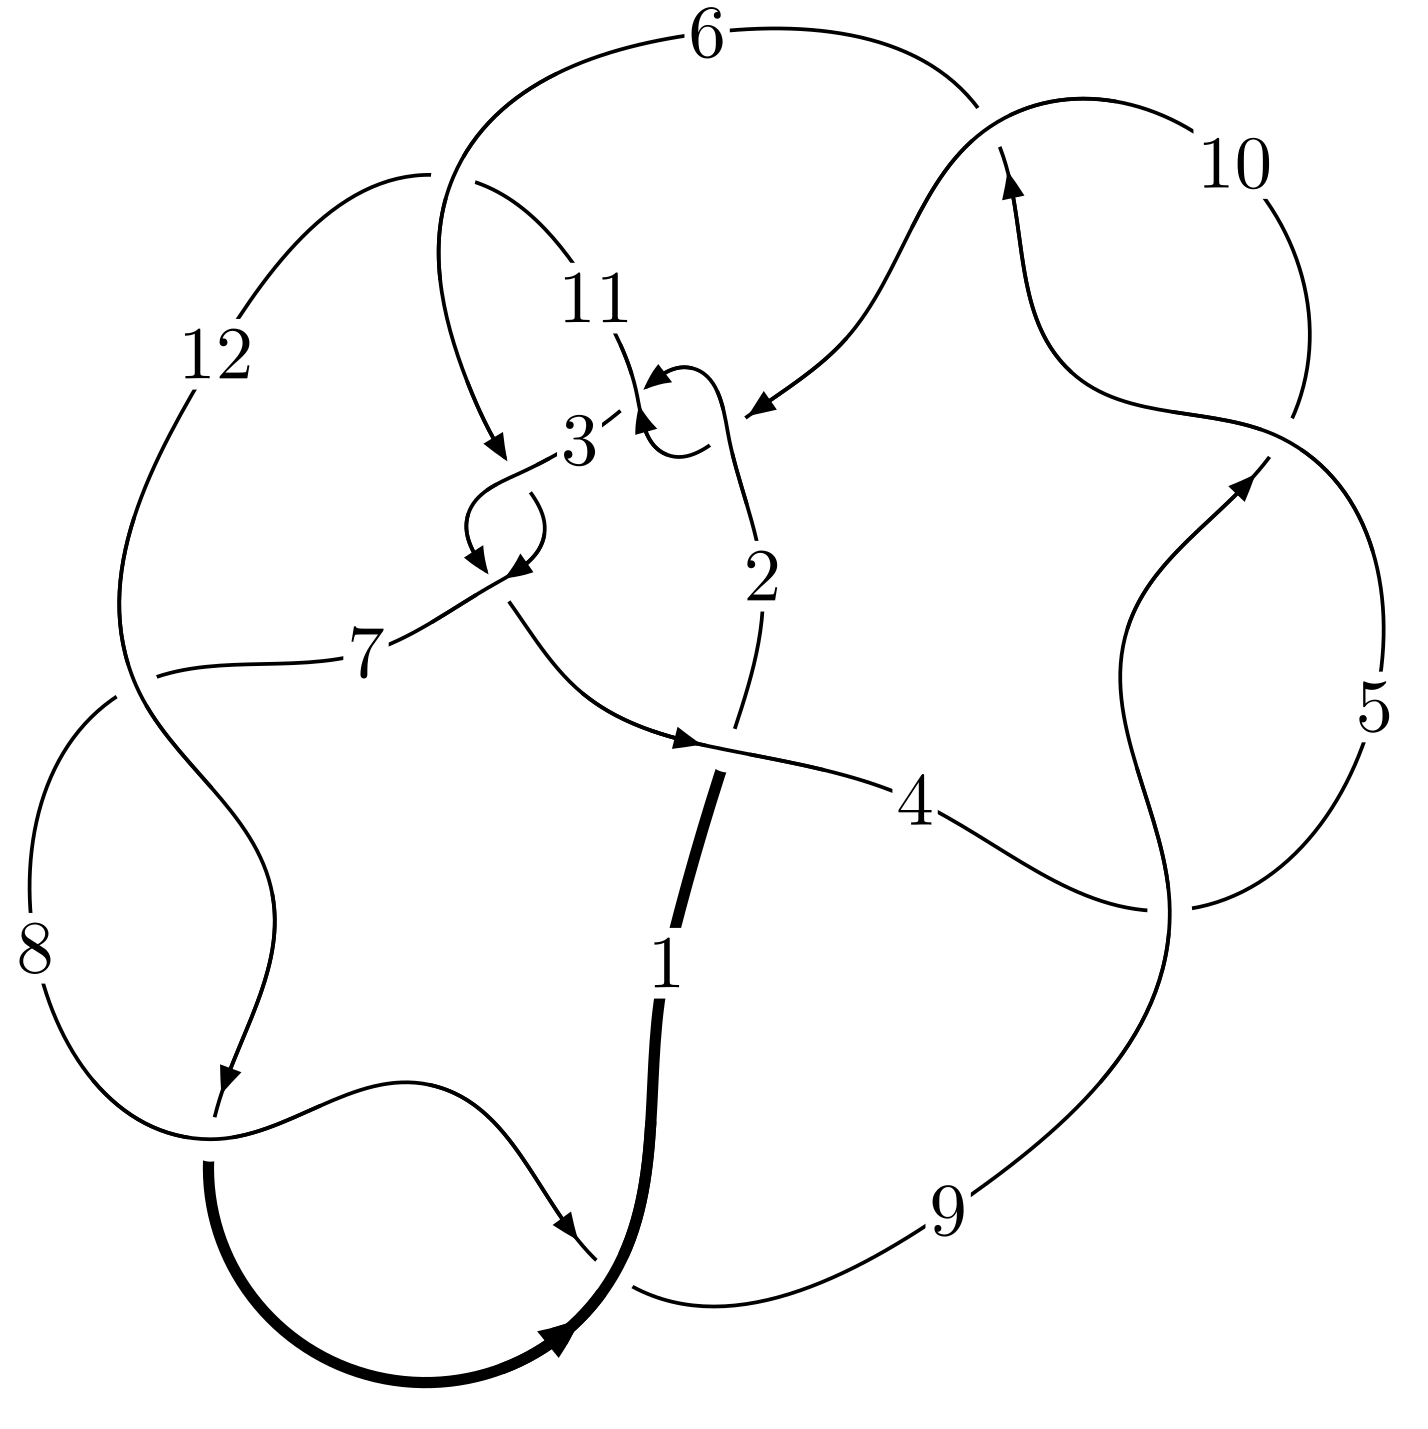
\includegraphics[width=112pt]{../../../GIT/diagram.site/Diagrams/png/2004_12a_1203.png}\\
\ \ \ A knot diagram\footnotemark}&
\allowdisplaybreaks
\textbf{Linearized knot diagam} \\
\cline{2-2}
 &
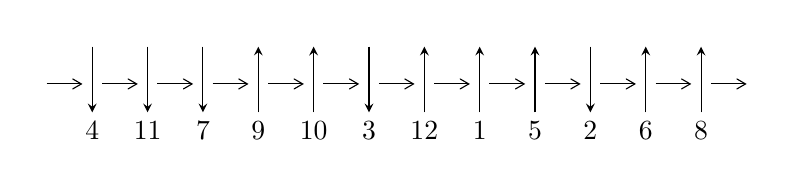
\begin{tikzpicture}[x=20pt, y=17pt]
	% nodes
	\node (C0) at (0, 0) {};
	\node (C1) at (1, 0) {};
	\node (C1U) at (1, +1) {};
	\node (C1D) at (1, -1) {4};

	\node (C2) at (2, 0) {};
	\node (C2U) at (2, +1) {};
	\node (C2D) at (2, -1) {11};

	\node (C3) at (3, 0) {};
	\node (C3U) at (3, +1) {};
	\node (C3D) at (3, -1) {7};

	\node (C4) at (4, 0) {};
	\node (C4U) at (4, +1) {};
	\node (C4D) at (4, -1) {9};

	\node (C5) at (5, 0) {};
	\node (C5U) at (5, +1) {};
	\node (C5D) at (5, -1) {10};

	\node (C6) at (6, 0) {};
	\node (C6U) at (6, +1) {};
	\node (C6D) at (6, -1) {3};

	\node (C7) at (7, 0) {};
	\node (C7U) at (7, +1) {};
	\node (C7D) at (7, -1) {12};

	\node (C8) at (8, 0) {};
	\node (C8U) at (8, +1) {};
	\node (C8D) at (8, -1) {1};

	\node (C9) at (9, 0) {};
	\node (C9U) at (9, +1) {};
	\node (C9D) at (9, -1) {5};

	\node (C10) at (10, 0) {};
	\node (C10U) at (10, +1) {};
	\node (C10D) at (10, -1) {2};

	\node (C11) at (11, 0) {};
	\node (C11U) at (11, +1) {};
	\node (C11D) at (11, -1) {6};

	\node (C12) at (12, 0) {};
	\node (C12U) at (12, +1) {};
	\node (C12D) at (12, -1) {8};
	\node (C13) at (13, 0) {};

	% arrows
	\draw[->,>={angle 60}]
	(C0) edge (C1) (C1) edge (C2) (C2) edge (C3) (C3) edge (C4) (C4) edge (C5) (C5) edge (C6) (C6) edge (C7) (C7) edge (C8) (C8) edge (C9) (C9) edge (C10) (C10) edge (C11) (C11) edge (C12) (C12) edge (C13) ;	\draw[->,>=stealth]
	(C1U) edge (C1D) (C2U) edge (C2D) (C3U) edge (C3D) (C4D) edge (C4U) (C5D) edge (C5U) (C6U) edge (C6D) (C7D) edge (C7U) (C8D) edge (C8U) (C9D) edge (C9U) (C10U) edge (C10D) (C11D) edge (C11U) (C12D) edge (C12U) ;
	\end{tikzpicture} \\
\hhline{~~} \\& 
\textbf{Solving Sequence} \\ \cline{2-2} 
 &
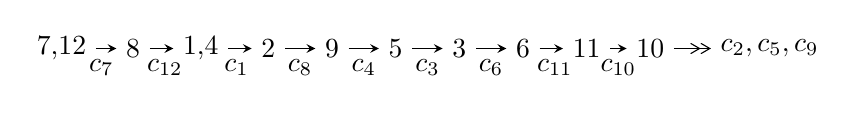
\begin{tikzpicture}[x=23pt, y=7pt]
	% node
	\node (A0) at (-1/8, 0) {7,12};
	\node (A1) at (1, 0) {8};
	\node (A2) at (33/16, 0) {1,4};
	\node (A3) at (25/8, 0) {2};
	\node (A4) at (33/8, 0) {9};
	\node (A5) at (41/8, 0) {5};
	\node (A6) at (49/8, 0) {3};
	\node (A7) at (57/8, 0) {6};
	\node (A8) at (65/8, 0) {11};
	\node (A9) at (73/8, 0) {10};
	\node (C1) at (1/2, -1) {$c_{7}$};
	\node (C2) at (3/2, -1) {$c_{12}$};
	\node (C3) at (21/8, -1) {$c_{1}$};
	\node (C4) at (29/8, -1) {$c_{8}$};
	\node (C5) at (37/8, -1) {$c_{4}$};
	\node (C6) at (45/8, -1) {$c_{3}$};
	\node (C7) at (53/8, -1) {$c_{6}$};
	\node (C8) at (61/8, -1) {$c_{11}$};
	\node (C9) at (69/8, -1) {$c_{10}$};
	\node (A10) at (11, 0) {$c_{2},c_{5},c_{9}$};

	% edge
	\draw[->,>=stealth]	
	(A0) edge (A1) (A1) edge (A2) (A2) edge (A3) (A3) edge (A4) (A4) edge (A5) (A5) edge (A6) (A6) edge (A7) (A7) edge (A8) (A8) edge (A9) ;
	\draw[->>,>={angle 60}]	
	(A9) edge (A10);
\end{tikzpicture} \\ 

\end{tabular} \\

\footnotetext{
The image of knot diagram is generated by the software ``\textbf{Draw programme}" developed by Andrew Bartholomew(\url{http://www.layer8.co.uk/maths/draw/index.htm\#Running-draw}), where we modified some parts for our purpose(\url{https://github.com/CATsTAILs/LinksPainter}).
}\phantom \\ \newline 
\centering \textbf{Ideals for irreducible components\footnotemark of $X_{\text{par}}$} 
 
\begin{align*}
I^u_{1}&=\langle 
4 u^{10}-2 u^9-23 u^8+12 u^7+42 u^6-23 u^5-20 u^4+20 u^3+b-16 u-6,\\
\phantom{I^u_{1}}&\phantom{= \langle  }-24 u^{10}+16 u^9+131 u^8-92 u^7-215 u^6+162 u^5+63 u^4-111 u^3+16 u^2+7 a+83 u+29,\\
\phantom{I^u_{1}}&\phantom{= \langle  }u^{11}-6 u^9+12 u^7-8 u^5+2 u^4+3 u^3-4 u^2-4 u-1\rangle \\
I^u_{2}&=\langle 
1.89277\times10^{85} u^{59}-8.97500\times10^{85} u^{58}+\cdots+5.45911\times10^{86} b+6.16613\times10^{86},\\
\phantom{I^u_{2}}&\phantom{= \langle  }-3.98384\times10^{87} u^{59}+1.21124\times10^{88} u^{58}+\cdots+1.63773\times10^{87} a-8.06741\times10^{86},\;u^{60}-3 u^{59}+\cdots-4 u+1\rangle \\
\\
\end{align*}
\raggedright * 2 irreducible components of $\dim_{\mathbb{C}}=0$, with total 71 representations.\\
\footnotetext{All coefficients of polynomials are rational numbers. But the coefficients are sometimes approximated in decimal forms when there is not enough margin.}
\newpage
\renewcommand{\arraystretch}{1}
\centering \section*{I. $I^u_{1}= \langle 4 u^{10}-2 u^9+\cdots+b-6,\;-24 u^{10}+16 u^9+\cdots+7 a+29,\;u^{11}-6 u^9+\cdots-4 u-1 \rangle$}
\flushleft \textbf{(i) Arc colorings}\\
\begin{tabular}{m{7pt} m{180pt} m{7pt} m{180pt} }
\flushright $a_{7}=$&$\begin{pmatrix}1\\0\end{pmatrix}$ \\
\flushright $a_{12}=$&$\begin{pmatrix}0\\u\end{pmatrix}$ \\
\flushright $a_{8}=$&$\begin{pmatrix}1\\- u^2\end{pmatrix}$ \\
\flushright $a_{1}=$&$\begin{pmatrix}u\\- u^3+u\end{pmatrix}$ \\
\flushright $a_{4}=$&$\begin{pmatrix}\frac{24}{7} u^{10}-\frac{16}{7} u^9+\cdots-\frac{83}{7} u-\frac{29}{7}\\-4 u^{10}+2 u^9+23 u^8-12 u^7-42 u^6+23 u^5+20 u^4-20 u^3+16 u+6\end{pmatrix}$ \\
\flushright $a_{2}=$&$\begin{pmatrix}-4.48980 u^{10}+4.32653 u^{9}+\cdots+17.8367 u+4.73469\\\frac{30}{7} u^{10}-\frac{20}{7} u^9+\cdots-\frac{109}{7} u-\frac{38}{7}\end{pmatrix}$ \\
\flushright $a_{9}=$&$\begin{pmatrix}- u^2+1\\u^4-2 u^2\end{pmatrix}$ \\
\flushright $a_{5}=$&$\begin{pmatrix}\frac{24}{7} u^{10}-\frac{16}{7} u^9+\cdots-\frac{76}{7} u-\frac{29}{7}\\-4 u^{10}+2 u^9+23 u^8-12 u^7-42 u^6+24 u^5+20 u^4-22 u^3+16 u+6\end{pmatrix}$ \\
\flushright $a_{3}=$&$\begin{pmatrix}-\frac{4}{7} u^{10}-\frac{2}{7} u^9+\cdots+\frac{29}{7} u+\frac{13}{7}\\-4 u^{10}+2 u^9+23 u^8-12 u^7-42 u^6+23 u^5+20 u^4-20 u^3+16 u+6\end{pmatrix}$ \\
\flushright $a_{6}=$&$\begin{pmatrix}-1.57143 u^{10}+1.71429 u^{9}+\cdots+4.14286 u+1.85714\\3 u^{10}-2 u^9+\cdots-12 u-4\end{pmatrix}$ \\
\flushright $a_{11}=$&$\begin{pmatrix}-1.65306 u^{10}+2.10204 u^{9}+\cdots-0.551020 u-1.02041\\\frac{33}{7} u^{10}-\frac{22}{7} u^9+\cdots-\frac{115}{7} u-\frac{39}{7}\end{pmatrix}$ \\
\flushright $a_{10}=$&$\begin{pmatrix}\frac{16}{7} u^{10}-\frac{13}{7} u^9+\cdots-\frac{67}{7} u-\frac{17}{7}\\-2 u^{10}+u^9+\cdots+10 u+4\end{pmatrix}$\\&\end{tabular}
\flushleft \textbf{(ii) Obstruction class $= -1$}\\~\\
\flushleft \textbf{(iii) Cusp Shapes $= \frac{68}{7} u^{10}-\frac{36}{7} u^9-\frac{384}{7} u^8+\frac{228}{7} u^7+\frac{664}{7} u^6-\frac{480}{7} u^5-32 u^4+\frac{444}{7} u^3-\frac{92}{7} u^2-\frac{276}{7} u-\frac{18}{7}$}\\~\\
\newpage\renewcommand{\arraystretch}{1}
\flushleft \textbf{(iv) u-Polynomials at the component}\newline \\
\begin{tabular}{m{50pt}|m{274pt}}
Crossings & \hspace{64pt}u-Polynomials at each crossing \\
\hline $$\begin{aligned}c_{1}\end{aligned}$$&$\begin{aligned}
&7(7 u^{11}-57 u^{10}+\cdots-288 u+64)
\end{aligned}$\\
\hline $$\begin{aligned}c_{2},c_{3},c_{6}\\c_{10}\end{aligned}$$&$\begin{aligned}
&u^{11}+2 u^{10}-2 u^9-6 u^8+6 u^6+6 u^5+4 u^4-3 u^3-2 u^2+2 u-1
\end{aligned}$\\
\hline $$\begin{aligned}c_{4},c_{5},c_{7}\\c_{8},c_{9},c_{12}\end{aligned}$$&$\begin{aligned}
&u^{11}-6 u^9+12 u^7-8 u^5-2 u^4+3 u^3+4 u^2-4 u+1
\end{aligned}$\\
\hline $$\begin{aligned}c_{11}\end{aligned}$$&$\begin{aligned}
&7(7 u^{11}-57 u^{10}+\cdots-1232 u+160)
\end{aligned}$\\
\hline
\end{tabular}\\~\\
\newpage\renewcommand{\arraystretch}{1}
\flushleft \textbf{(v) Riley Polynomials at the component}\newline \\
\begin{tabular}{m{50pt}|m{274pt}}
Crossings & \hspace{64pt}Riley Polynomials at each crossing \\
\hline $$\begin{aligned}c_{1}\end{aligned}$$&$\begin{aligned}
&49(49 y^{11}-141 y^{10}+\cdots-48128 y-4096)
\end{aligned}$\\
\hline $$\begin{aligned}c_{2},c_{3},c_{6}\\c_{10}\end{aligned}$$&$\begin{aligned}
&y^{11}-8 y^{10}+\cdots-8 y^2-1
\end{aligned}$\\
\hline $$\begin{aligned}c_{4},c_{5},c_{7}\\c_{8},c_{9},c_{12}\end{aligned}$$&$\begin{aligned}
&y^{11}-12 y^{10}+\cdots+8 y-1
\end{aligned}$\\
\hline $$\begin{aligned}c_{11}\end{aligned}$$&$\begin{aligned}
&49(49 y^{11}-575 y^{10}+\cdots+214784 y-25600)
\end{aligned}$\\
\hline
\end{tabular}\\~\\
\newpage\flushleft \textbf{(vi) Complex Volumes and Cusp Shapes}
$$\begin{array}{c|c|c}  
\text{Solutions to }I^u_{1}& \I (\text{vol} + \sqrt{-1}CS) & \text{Cusp shape}\\
 \hline 
\begin{aligned}
u &= \phantom{-}0.478687 + 0.745648 I \\
a &= -0.553902 - 0.948598 I \\
b &= -1.34136 + 0.45173 I\end{aligned}
 & -5.83345 + 8.24192 I & -1.78003 - 8.25664 I \\ \hline\begin{aligned}
u &= \phantom{-}0.478687 - 0.745648 I \\
a &= -0.553902 + 0.948598 I \\
b &= -1.34136 - 0.45173 I\end{aligned}
 & -5.83345 - 8.24192 I & -1.78003 + 8.25664 I \\ \hline\begin{aligned}
u &= -0.658231 + 0.262357 I \\
a &= -1.46305 - 1.04015 I \\
b &= \phantom{-}1.266780 - 0.115508 I\end{aligned}
 & -4.39476 + 0.14427 I & \phantom{-}2.57188 + 3.97363 I \\ \hline\begin{aligned}
u &= -0.658231 - 0.262357 I \\
a &= -1.46305 + 1.04015 I \\
b &= \phantom{-}1.266780 + 0.115508 I\end{aligned}
 & -4.39476 - 0.14427 I & \phantom{-}2.57188 - 3.97363 I \\ \hline\begin{aligned}
u &= \phantom{-}1.33602\phantom{ +0.000000I} \\
a &= \phantom{-}2.25023\phantom{ +0.000000I} \\
b &= -0.601613\phantom{ +0.000000I}\end{aligned}
 & \phantom{-}7.19259\phantom{ +0.000000I} & \phantom{-}15.0510\phantom{ +0.000000I} \\ \hline\begin{aligned}
u &= -0.479037 + 0.241898 I \\
a &= -0.181635 - 0.272909 I \\
b &= -0.259055 + 0.400626 I\end{aligned}
 & \phantom{-}0.928640 - 0.385456 I & \phantom{-}9.67201 + 2.53338 I \\ \hline\begin{aligned}
u &= -0.479037 - 0.241898 I \\
a &= -0.181635 + 0.272909 I \\
b &= -0.259055 - 0.400626 I\end{aligned}
 & \phantom{-}0.928640 + 0.385456 I & \phantom{-}9.67201 - 2.53338 I \\ \hline\begin{aligned}
u &= -1.58856 + 0.17840 I \\
a &= -0.206594 + 1.159350 I \\
b &= \phantom{-}0.242301 - 0.964246 I\end{aligned}
 & \phantom{-}15.1584 - 4.3999 I & \phantom{-}11.24843 + 1.35382 I \\ \hline\begin{aligned}
u &= -1.58856 - 0.17840 I \\
a &= -0.206594 - 1.159350 I \\
b &= \phantom{-}0.242301 + 0.964246 I\end{aligned}
 & \phantom{-}15.1584 + 4.3999 I & \phantom{-}11.24843 - 1.35382 I \\ \hline\begin{aligned}
u &= \phantom{-}1.57913 + 0.29390 I \\
a &= -0.36279 + 1.54535 I \\
b &= \phantom{-}1.39214 - 0.58407 I\end{aligned}
 & \phantom{-}7.8167 + 16.1195 I & \phantom{-}5.19082 - 7.65707 I\\
 \hline 
 \end{array}$$\newpage$$\begin{array}{c|c|c}  
\text{Solutions to }I^u_{1}& \I (\text{vol} + \sqrt{-1}CS) & \text{Cusp shape}\\
 \hline 
\begin{aligned}
u &= \phantom{-}1.57913 - 0.29390 I \\
a &= -0.36279 - 1.54535 I \\
b &= \phantom{-}1.39214 + 0.58407 I\end{aligned}
 & \phantom{-}7.8167 - 16.1195 I & \phantom{-}5.19082 + 7.65707 I\\
 \hline 
 \end{array}$$\newpage\newpage\renewcommand{\arraystretch}{1}
\centering \section*{II. $I^u_{2}= \langle 1.89\times10^{85} u^{59}-8.98\times10^{85} u^{58}+\cdots+5.46\times10^{86} b+6.17\times10^{86},\;-3.98\times10^{87} u^{59}+1.21\times10^{88} u^{58}+\cdots+1.64\times10^{87} a-8.07\times10^{86},\;u^{60}-3 u^{59}+\cdots-4 u+1 \rangle$}
\flushleft \textbf{(i) Arc colorings}\\
\begin{tabular}{m{7pt} m{180pt} m{7pt} m{180pt} }
\flushright $a_{7}=$&$\begin{pmatrix}1\\0\end{pmatrix}$ \\
\flushright $a_{12}=$&$\begin{pmatrix}0\\u\end{pmatrix}$ \\
\flushright $a_{8}=$&$\begin{pmatrix}1\\- u^2\end{pmatrix}$ \\
\flushright $a_{1}=$&$\begin{pmatrix}u\\- u^3+u\end{pmatrix}$ \\
\flushright $a_{4}=$&$\begin{pmatrix}2.43253 u^{59}-7.39586 u^{58}+\cdots-72.0815 u+0.492596\\-0.0346718 u^{59}+0.164404 u^{58}+\cdots-0.741074 u-1.12951\end{pmatrix}$ \\
\flushright $a_{2}=$&$\begin{pmatrix}8.63257 u^{59}-26.7187 u^{58}+\cdots-207.349 u+18.6317\\-0.243987 u^{59}+0.846358 u^{58}+\cdots+9.95097 u-2.79898\end{pmatrix}$ \\
\flushright $a_{9}=$&$\begin{pmatrix}- u^2+1\\u^4-2 u^2\end{pmatrix}$ \\
\flushright $a_{5}=$&$\begin{pmatrix}2.76707 u^{59}-8.30435 u^{58}+\cdots-79.3106 u-0.0929557\\-0.0306498 u^{59}+0.143629 u^{58}+\cdots-0.263022 u-1.12429\end{pmatrix}$ \\
\flushright $a_{3}=$&$\begin{pmatrix}2.39786 u^{59}-7.23146 u^{58}+\cdots-72.8226 u-0.636916\\-0.0346718 u^{59}+0.164404 u^{58}+\cdots-0.741074 u-1.12951\end{pmatrix}$ \\
\flushright $a_{6}=$&$\begin{pmatrix}3.00540 u^{59}-9.41833 u^{58}+\cdots-57.5152 u-3.02190\\0.197053 u^{59}-0.528407 u^{58}+\cdots+0.476650 u-1.12091\end{pmatrix}$ \\
\flushright $a_{11}=$&$\begin{pmatrix}6.13879 u^{59}-20.4327 u^{58}+\cdots-157.725 u+8.37417\\-0.446686 u^{59}+1.03858 u^{58}+\cdots+5.09039 u-2.20303\end{pmatrix}$ \\
\flushright $a_{10}=$&$\begin{pmatrix}-0.616946 u^{59}+2.65559 u^{58}+\cdots+44.4296 u-20.2992\\0.144193 u^{59}-0.493218 u^{58}+\cdots-8.00218 u-0.368881\end{pmatrix}$\\&\end{tabular}
\flushleft \textbf{(ii) Obstruction class $= -1$}\\~\\
\flushleft \textbf{(iii) Cusp Shapes $= 4.59968 u^{59}-12.3313 u^{58}+\cdots-95.2581 u+14.2700$}\\~\\
\newpage\renewcommand{\arraystretch}{1}
\flushleft \textbf{(iv) u-Polynomials at the component}\newline \\
\begin{tabular}{m{50pt}|m{274pt}}
Crossings & \hspace{64pt}u-Polynomials at each crossing \\
\hline $$\begin{aligned}c_{1}\end{aligned}$$&$\begin{aligned}
&9(3 u^{30}+36 u^{29}+\cdots+154 u-41)^{2}
\end{aligned}$\\
\hline $$\begin{aligned}c_{2},c_{3},c_{6}\\c_{10}\end{aligned}$$&$\begin{aligned}
&u^{60}- u^{59}+\cdots-14 u+1
\end{aligned}$\\
\hline $$\begin{aligned}c_{4},c_{5},c_{7}\\c_{8},c_{9},c_{12}\end{aligned}$$&$\begin{aligned}
&u^{60}+3 u^{59}+\cdots+4 u+1
\end{aligned}$\\
\hline $$\begin{aligned}c_{11}\end{aligned}$$&$\begin{aligned}
&9(3 u^{30}-3 u^{29}+\cdots+15 u+1)^{2}
\end{aligned}$\\
\hline
\end{tabular}\\~\\
\newpage\renewcommand{\arraystretch}{1}
\flushleft \textbf{(v) Riley Polynomials at the component}\newline \\
\begin{tabular}{m{50pt}|m{274pt}}
Crossings & \hspace{64pt}Riley Polynomials at each crossing \\
\hline $$\begin{aligned}c_{1}\end{aligned}$$&$\begin{aligned}
&81(9 y^{30}-102 y^{29}+\cdots-66274 y+1681)^{2}
\end{aligned}$\\
\hline $$\begin{aligned}c_{2},c_{3},c_{6}\\c_{10}\end{aligned}$$&$\begin{aligned}
&y^{60}-37 y^{59}+\cdots-428 y+1
\end{aligned}$\\
\hline $$\begin{aligned}c_{4},c_{5},c_{7}\\c_{8},c_{9},c_{12}\end{aligned}$$&$\begin{aligned}
&y^{60}-61 y^{59}+\cdots-68 y+1
\end{aligned}$\\
\hline $$\begin{aligned}c_{11}\end{aligned}$$&$\begin{aligned}
&81(9 y^{30}-147 y^{29}+\cdots-69 y+1)^{2}
\end{aligned}$\\
\hline
\end{tabular}\\~\\
\newpage\flushleft \textbf{(vi) Complex Volumes and Cusp Shapes}
$$\begin{array}{c|c|c}  
\text{Solutions to }I^u_{2}& \I (\text{vol} + \sqrt{-1}CS) & \text{Cusp shape}\\
 \hline 
\begin{aligned}
u &= \phantom{-}0.833474 + 0.555513 I \\
a &= \phantom{-}0.387187 - 0.319977 I \\
b &= \phantom{-}0.185112 + 0.453484 I\end{aligned}
 & \phantom{-}7.21827 + 1.60938 I & \phantom{-0.000000 } 0 \\ \hline\begin{aligned}
u &= \phantom{-}0.833474 - 0.555513 I \\
a &= \phantom{-}0.387187 + 0.319977 I \\
b &= \phantom{-}0.185112 - 0.453484 I\end{aligned}
 & \phantom{-}7.21827 - 1.60938 I & \phantom{-0.000000 } 0 \\ \hline\begin{aligned}
u &= \phantom{-}0.620080 + 0.732888 I \\
a &= \phantom{-}0.027446 - 0.613448 I \\
b &= -1.204640 - 0.259326 I\end{aligned}
 & -5.45352 - 3.30155 I & \phantom{-0.000000 } 0 \\ \hline\begin{aligned}
u &= \phantom{-}0.620080 - 0.732888 I \\
a &= \phantom{-}0.027446 + 0.613448 I \\
b &= -1.204640 + 0.259326 I\end{aligned}
 & -5.45352 + 3.30155 I & \phantom{-0.000000 } 0 \\ \hline\begin{aligned}
u &= -0.629559 + 0.862226 I \\
a &= \phantom{-}0.486783 - 1.011150 I \\
b &= \phantom{-}1.315580 + 0.457135 I\end{aligned}
 & \phantom{-}0.61217 - 11.85690 I & \phantom{-0.000000 } 0 \\ \hline\begin{aligned}
u &= -0.629559 - 0.862226 I \\
a &= \phantom{-}0.486783 + 1.011150 I \\
b &= \phantom{-}1.315580 - 0.457135 I\end{aligned}
 & \phantom{-}0.61217 + 11.85690 I & \phantom{-0.000000 } 0 \\ \hline\begin{aligned}
u &= -0.363141 + 0.797919 I \\
a &= -0.719921 + 0.642225 I \\
b &= -1.011050 - 0.278044 I\end{aligned}
 & -1.08758 - 3.25958 I & \phantom{-}2.38011 + 10.20080 I \\ \hline\begin{aligned}
u &= -0.363141 - 0.797919 I \\
a &= -0.719921 - 0.642225 I \\
b &= -1.011050 + 0.278044 I\end{aligned}
 & -1.08758 + 3.25958 I & \phantom{-}2.38011 - 10.20080 I \\ \hline\begin{aligned}
u &= -0.647832 + 0.589870 I \\
a &= -0.129345 + 0.669989 I \\
b &= -0.089131 - 0.919019 I\end{aligned}
 & \phantom{-}4.91596 - 6.95691 I & \phantom{-}6.13134 + 6.91488 I \\ \hline\begin{aligned}
u &= -0.647832 - 0.589870 I \\
a &= -0.129345 - 0.669989 I \\
b &= -0.089131 + 0.919019 I\end{aligned}
 & \phantom{-}4.91596 + 6.95691 I & \phantom{-}6.13134 - 6.91488 I\\
 \hline 
 \end{array}$$\newpage$$\begin{array}{c|c|c}  
\text{Solutions to }I^u_{2}& \I (\text{vol} + \sqrt{-1}CS) & \text{Cusp shape}\\
 \hline 
\begin{aligned}
u &= -0.560987 + 1.036060 I \\
a &= \phantom{-}0.195707 - 0.202609 I \\
b &= \phantom{-}1.166400 - 0.314203 I\end{aligned}
 & \phantom{-}0.26680 + 5.75700 I & \phantom{-0.000000 } 0 \\ \hline\begin{aligned}
u &= -0.560987 - 1.036060 I \\
a &= \phantom{-}0.195707 + 0.202609 I \\
b &= \phantom{-}1.166400 + 0.314203 I\end{aligned}
 & \phantom{-}0.26680 - 5.75700 I & \phantom{-0.000000 } 0 \\ \hline\begin{aligned}
u &= -0.228769 + 0.724317 I \\
a &= \phantom{-}1.003230 - 0.131008 I \\
b &= -0.044280 + 0.505989 I\end{aligned}
 & \phantom{-}3.67376 + 2.63649 I & \phantom{-}5.81236 - 1.84652 I \\ \hline\begin{aligned}
u &= -0.228769 - 0.724317 I \\
a &= \phantom{-}1.003230 + 0.131008 I \\
b &= -0.044280 - 0.505989 I\end{aligned}
 & \phantom{-}3.67376 - 2.63649 I & \phantom{-}5.81236 + 1.84652 I \\ \hline\begin{aligned}
u &= \phantom{-}0.579713 + 1.108340 I \\
a &= \phantom{-}0.470071 + 0.518344 I \\
b &= \phantom{-}1.000490 - 0.320542 I\end{aligned}
 & \phantom{-}5.13933 + 4.75641 I & \phantom{-0.000000 } 0 \\ \hline\begin{aligned}
u &= \phantom{-}0.579713 - 1.108340 I \\
a &= \phantom{-}0.470071 - 0.518344 I \\
b &= \phantom{-}1.000490 + 0.320542 I\end{aligned}
 & \phantom{-}5.13933 - 4.75641 I & \phantom{-0.000000 } 0 \\ \hline\begin{aligned}
u &= \phantom{-}1.357920 + 0.019295 I \\
a &= \phantom{-}1.84637 + 0.92508 I \\
b &= \phantom{-}1.066870 - 0.034317 I\end{aligned}
 & \phantom{-}1.55370 + 0.00608 I & \phantom{-0.000000 } 0 \\ \hline\begin{aligned}
u &= \phantom{-}1.357920 - 0.019295 I \\
a &= \phantom{-}1.84637 - 0.92508 I \\
b &= \phantom{-}1.066870 + 0.034317 I\end{aligned}
 & \phantom{-}1.55370 - 0.00608 I & \phantom{-0.000000 } 0 \\ \hline\begin{aligned}
u &= -0.325223 + 0.548272 I \\
a &= \phantom{-}0.643224 - 0.820076 I \\
b &= \phantom{-}1.39941 + 0.44826 I\end{aligned}
 & -5.45352 - 3.30155 I & -2.99005 + 4.83446 I \\ \hline\begin{aligned}
u &= -0.325223 - 0.548272 I \\
a &= \phantom{-}0.643224 + 0.820076 I \\
b &= \phantom{-}1.39941 - 0.44826 I\end{aligned}
 & -5.45352 + 3.30155 I & -2.99005 - 4.83446 I\\
 \hline 
 \end{array}$$\newpage$$\begin{array}{c|c|c}  
\text{Solutions to }I^u_{2}& \I (\text{vol} + \sqrt{-1}CS) & \text{Cusp shape}\\
 \hline 
\begin{aligned}
u &= -1.38075 + 0.35680 I \\
a &= -0.068945 + 0.802649 I \\
b &= -0.934678 - 0.203671 I\end{aligned}
 & \phantom{-}1.87339 - 1.59238 I & \phantom{-0.000000 } 0 \\ \hline\begin{aligned}
u &= -1.38075 - 0.35680 I \\
a &= -0.068945 - 0.802649 I \\
b &= -0.934678 + 0.203671 I\end{aligned}
 & \phantom{-}1.87339 + 1.59238 I & \phantom{-0.000000 } 0 \\ \hline\begin{aligned}
u &= -1.42198 + 0.11012 I \\
a &= -0.49563 - 1.58905 I \\
b &= \phantom{-}0.999372 + 0.593646 I\end{aligned}
 & \phantom{-}3.67376 - 2.63649 I & \phantom{-0.000000 } 0 \\ \hline\begin{aligned}
u &= -1.42198 - 0.11012 I \\
a &= -0.49563 + 1.58905 I \\
b &= \phantom{-}0.999372 - 0.593646 I\end{aligned}
 & \phantom{-}3.67376 + 2.63649 I & \phantom{-0.000000 } 0 \\ \hline\begin{aligned}
u &= -1.44134\phantom{ +0.000000I} \\
a &= -0.648369\phantom{ +0.000000I} \\
b &= -0.0486569\phantom{ +0.000000I}\end{aligned}
 & \phantom{-}3.34318\phantom{ +0.000000I} & \phantom{-0.000000 } 0 \\ \hline\begin{aligned}
u &= \phantom{-}0.428325 + 0.345067 I \\
a &= \phantom{-}0.117620 + 0.589809 I \\
b &= \phantom{-}0.243272 - 0.979166 I\end{aligned}
 & -1.08758 + 3.25958 I & \phantom{-}2.38011 - 10.20080 I \\ \hline\begin{aligned}
u &= \phantom{-}0.428325 - 0.345067 I \\
a &= \phantom{-}0.117620 - 0.589809 I \\
b &= \phantom{-}0.243272 + 0.979166 I\end{aligned}
 & -1.08758 - 3.25958 I & \phantom{-}2.38011 + 10.20080 I \\ \hline\begin{aligned}
u &= \phantom{-}1.44300 + 0.15336 I \\
a &= -0.82586 + 1.54444 I \\
b &= \phantom{-}1.51584 - 0.77183 I\end{aligned}
 & \phantom{-}0.26680 + 5.75700 I & \phantom{-0.000000 } 0 \\ \hline\begin{aligned}
u &= \phantom{-}1.44300 - 0.15336 I \\
a &= -0.82586 - 1.54444 I \\
b &= \phantom{-}1.51584 + 0.77183 I\end{aligned}
 & \phantom{-}0.26680 - 5.75700 I & \phantom{-0.000000 } 0 \\ \hline\begin{aligned}
u &= -1.46078\phantom{ +0.000000I} \\
a &= \phantom{-}0.376305\phantom{ +0.000000I} \\
b &= -1.57915\phantom{ +0.000000I}\end{aligned}
 & \phantom{-}8.95550\phantom{ +0.000000I} & \phantom{-0.000000 } 0\\
 \hline 
 \end{array}$$\newpage$$\begin{array}{c|c|c}  
\text{Solutions to }I^u_{2}& \I (\text{vol} + \sqrt{-1}CS) & \text{Cusp shape}\\
 \hline 
\begin{aligned}
u &= \phantom{-}1.47066 + 0.07345 I \\
a &= \phantom{-}0.445781 + 1.290480 I \\
b &= -0.446296 - 0.915918 I\end{aligned}
 & \phantom{-}7.21827 + 1.60938 I & \phantom{-0.000000 } 0 \\ \hline\begin{aligned}
u &= \phantom{-}1.47066 - 0.07345 I \\
a &= \phantom{-}0.445781 - 1.290480 I \\
b &= -0.446296 + 0.915918 I\end{aligned}
 & \phantom{-}7.21827 - 1.60938 I & \phantom{-0.000000 } 0 \\ \hline\begin{aligned}
u &= -1.47406\phantom{ +0.000000I} \\
a &= \phantom{-}0.939294\phantom{ +0.000000I} \\
b &= -1.86730\phantom{ +0.000000I}\end{aligned}
 & \phantom{-}8.91513\phantom{ +0.000000I} & \phantom{-0.000000 } 0 \\ \hline\begin{aligned}
u &= -1.47658 + 0.08795 I \\
a &= \phantom{-}0.08740 - 1.86794 I \\
b &= \phantom{-}0.11923 + 1.50677 I\end{aligned}
 & \phantom{-}5.13933 - 4.75641 I & \phantom{-0.000000 } 0 \\ \hline\begin{aligned}
u &= -1.47658 - 0.08795 I \\
a &= \phantom{-}0.08740 + 1.86794 I \\
b &= \phantom{-}0.11923 - 1.50677 I\end{aligned}
 & \phantom{-}5.13933 + 4.75641 I & \phantom{-0.000000 } 0 \\ \hline\begin{aligned}
u &= \phantom{-}1.47858 + 0.04341 I \\
a &= \phantom{-}1.06994 + 1.32208 I \\
b &= -1.47842 - 1.04389 I\end{aligned}
 & \phantom{-}8.05603 + 2.43541 I & \phantom{-0.000000 } 0 \\ \hline\begin{aligned}
u &= \phantom{-}1.47858 - 0.04341 I \\
a &= \phantom{-}1.06994 - 1.32208 I \\
b &= -1.47842 + 1.04389 I\end{aligned}
 & \phantom{-}8.05603 - 2.43541 I & \phantom{-0.000000 } 0 \\ \hline\begin{aligned}
u &= \phantom{-}1.47684 + 0.25365 I \\
a &= \phantom{-}0.22074 - 1.43458 I \\
b &= -1.134910 + 0.555153 I\end{aligned}
 & \phantom{-}4.91596 + 6.95691 I & \phantom{-0.000000 } 0 \\ \hline\begin{aligned}
u &= \phantom{-}1.47684 - 0.25365 I \\
a &= \phantom{-}0.22074 + 1.43458 I \\
b &= -1.134910 - 0.555153 I\end{aligned}
 & \phantom{-}4.91596 - 6.95691 I & \phantom{-0.000000 } 0 \\ \hline\begin{aligned}
u &= -1.50444 + 0.25222 I \\
a &= \phantom{-}0.51791 + 1.58138 I \\
b &= -1.40913 - 0.64393 I\end{aligned}
 & \phantom{-}0.61217 - 11.85690 I & \phantom{-0.000000 } 0\\
 \hline 
 \end{array}$$\newpage$$\begin{array}{c|c|c}  
\text{Solutions to }I^u_{2}& \I (\text{vol} + \sqrt{-1}CS) & \text{Cusp shape}\\
 \hline 
\begin{aligned}
u &= -1.50444 - 0.25222 I \\
a &= \phantom{-}0.51791 - 1.58138 I \\
b &= -1.40913 + 0.64393 I\end{aligned}
 & \phantom{-}0.61217 + 11.85690 I & \phantom{-0.000000 } 0 \\ \hline\begin{aligned}
u &= -0.397490 + 0.226483 I \\
a &= -0.256525 - 0.636041 I \\
b &= -1.108750 + 0.697445 I\end{aligned}
 & \phantom{-}1.87339 - 1.59238 I & \phantom{-}6.67632 + 9.14419 I \\ \hline\begin{aligned}
u &= -0.397490 - 0.226483 I \\
a &= -0.256525 + 0.636041 I \\
b &= -1.108750 - 0.697445 I\end{aligned}
 & \phantom{-}1.87339 + 1.59238 I & \phantom{-}6.67632 - 9.14419 I \\ \hline\begin{aligned}
u &= \phantom{-}0.220469 + 0.386151 I \\
a &= \phantom{-}0.88338 + 1.75647 I \\
b &= \phantom{-}0.976188 - 0.197719 I\end{aligned}
 & -1.65573 + 0.87357 I & -2.51974 + 1.49849 I \\ \hline\begin{aligned}
u &= \phantom{-}0.220469 - 0.386151 I \\
a &= \phantom{-}0.88338 - 1.75647 I \\
b &= \phantom{-}0.976188 + 0.197719 I\end{aligned}
 & -1.65573 - 0.87357 I & -2.51974 - 1.49849 I \\ \hline\begin{aligned}
u &= \phantom{-}0.221492 + 0.372642 I \\
a &= -1.74604 + 0.73502 I \\
b &= \phantom{-}0.134818 + 0.350741 I\end{aligned}
 & -1.65573 - 0.87357 I & -2.51974 - 1.49849 I \\ \hline\begin{aligned}
u &= \phantom{-}0.221492 - 0.372642 I \\
a &= -1.74604 - 0.73502 I \\
b &= \phantom{-}0.134818 - 0.350741 I\end{aligned}
 & -1.65573 + 0.87357 I & -2.51974 + 1.49849 I \\ \hline\begin{aligned}
u &= \phantom{-}1.56045 + 0.18740 I \\
a &= -0.25231 - 1.52828 I \\
b &= -0.028871 + 1.223480 I\end{aligned}
 & \phantom{-}12.2304 + 9.8327 I & \phantom{-0.000000 } 0 \\ \hline\begin{aligned}
u &= \phantom{-}1.56045 - 0.18740 I \\
a &= -0.25231 + 1.52828 I \\
b &= -0.028871 - 1.223480 I\end{aligned}
 & \phantom{-}12.2304 - 9.8327 I & \phantom{-0.000000 } 0 \\ \hline\begin{aligned}
u &= \phantom{-}0.376786\phantom{ +0.000000I} \\
a &= -1.32121\phantom{ +0.000000I} \\
b &= -1.51840\phantom{ +0.000000I}\end{aligned}
 & \phantom{-}2.79630\phantom{ +0.000000I} & \phantom{-}14.5100\phantom{ +0.000000I}\\
 \hline 
 \end{array}$$\newpage$$\begin{array}{c|c|c}  
\text{Solutions to }I^u_{2}& \I (\text{vol} + \sqrt{-1}CS) & \text{Cusp shape}\\
 \hline 
\begin{aligned}
u &= -1.59069 + 0.33885 I \\
a &= -0.156905 - 1.268360 I \\
b &= \phantom{-}1.189620 + 0.558071 I\end{aligned}
 & \phantom{-}12.2304 - 9.8327 I & \phantom{-0.000000 } 0 \\ \hline\begin{aligned}
u &= -1.59069 - 0.33885 I \\
a &= -0.156905 + 1.268360 I \\
b &= \phantom{-}1.189620 - 0.558071 I\end{aligned}
 & \phantom{-}12.2304 + 9.8327 I & \phantom{-0.000000 } 0 \\ \hline\begin{aligned}
u &= -1.65135\phantom{ +0.000000I} \\
a &= \phantom{-}0.528394\phantom{ +0.000000I} \\
b &= -0.824716\phantom{ +0.000000I}\end{aligned}
 & \phantom{-}2.79630\phantom{ +0.000000I} & \phantom{-0.000000 } 0 \\ \hline\begin{aligned}
u &= \phantom{-}1.68306\phantom{ +0.000000I} \\
a &= \phantom{-}0.372386\phantom{ +0.000000I} \\
b &= \phantom{-}0.317785\phantom{ +0.000000I}\end{aligned}
 & \phantom{-}8.95550\phantom{ +0.000000I} & \phantom{-0.000000 } 0 \\ \hline\begin{aligned}
u &= -0.282510 + 0.079111 I \\
a &= \phantom{-}10.61020 + 7.07723 I \\
b &= -0.816929 - 0.088924 I\end{aligned}
 & \phantom{-}1.55370 + 0.00608 I & \phantom{-}23.9533 + 12.6442 I \\ \hline\begin{aligned}
u &= -0.282510 - 0.079111 I \\
a &= \phantom{-}10.61020 - 7.07723 I \\
b &= -0.816929 + 0.088924 I\end{aligned}
 & \phantom{-}1.55370 - 0.00608 I & \phantom{-}23.9533 - 12.6442 I \\ \hline\begin{aligned}
u &= \phantom{-}1.60577 + 0.59025 I \\
a &= \phantom{-}0.094048 + 0.587595 I \\
b &= \phantom{-}0.866646 - 0.256018 I\end{aligned}
 & \phantom{-}8.05603 + 2.43541 I & \phantom{-0.000000 } 0 \\ \hline\begin{aligned}
u &= \phantom{-}1.60577 - 0.59025 I \\
a &= \phantom{-}0.094048 - 0.587595 I \\
b &= \phantom{-}0.866646 + 0.256018 I\end{aligned}
 & \phantom{-}8.05603 - 2.43541 I & \phantom{-0.000000 } 0 \\ \hline\begin{aligned}
u &= \phantom{-}1.83729\phantom{ +0.000000I} \\
a &= -0.0147378\phantom{ +0.000000I} \\
b &= \phantom{-}0.649298\phantom{ +0.000000I}\end{aligned}
 & \phantom{-}8.91513\phantom{ +0.000000I} & \phantom{-0.000000 } 0 \\ \hline\begin{aligned}
u &= \phantom{-}0.156757\phantom{ +0.000000I} \\
a &= -8.14324\phantom{ +0.000000I} \\
b &= -1.07240\phantom{ +0.000000I}\end{aligned}
 & \phantom{-}3.34318\phantom{ +0.000000I} & \phantom{-}2.41920\phantom{ +0.000000I}\\
 \hline 
 \end{array}$$\newpage
\newpage\renewcommand{\arraystretch}{1}
\centering \section*{ III. u-Polynomials}
\begin{tabular}{m{50pt}|m{274pt}}
Crossings & \hspace{64pt}u-Polynomials at each crossing \\
\hline $$\begin{aligned}c_{1}\end{aligned}$$&$\begin{aligned}
&63(7 u^{11}-57 u^{10}+\cdots-288 u+64)\\
&\cdot(3 u^{30}+36 u^{29}+\cdots+154 u-41)^{2}
\end{aligned}$\\
\hline $$\begin{aligned}c_{2},c_{3},c_{6}\\c_{10}\end{aligned}$$&$\begin{aligned}
&(u^{11}+2 u^{10}-2 u^9-6 u^8+6 u^6+6 u^5+4 u^4-3 u^3-2 u^2+2 u-1)\\
&\cdot(u^{60}- u^{59}+\cdots-14 u+1)
\end{aligned}$\\
\hline $$\begin{aligned}c_{4},c_{5},c_{7}\\c_{8},c_{9},c_{12}\end{aligned}$$&$\begin{aligned}
&(u^{11}-6 u^9+12 u^7-8 u^5-2 u^4+3 u^3+4 u^2-4 u+1)\\
&\cdot(u^{60}+3 u^{59}+\cdots+4 u+1)
\end{aligned}$\\
\hline $$\begin{aligned}c_{11}\end{aligned}$$&$\begin{aligned}
&63(7 u^{11}-57 u^{10}+\cdots-1232 u+160)(3 u^{30}-3 u^{29}+\cdots+15 u+1)^{2}
\end{aligned}$\\
\hline
\end{tabular}\newpage\renewcommand{\arraystretch}{1}
\centering \section*{ IV. Riley Polynomials}
\begin{tabular}{m{50pt}|m{274pt}}
Crossings & \hspace{64pt}Riley Polynomials at each crossing \\
\hline $$\begin{aligned}c_{1}\end{aligned}$$&$\begin{aligned}
&3969(49 y^{11}-141 y^{10}+\cdots-48128 y-4096)\\
&\cdot(9 y^{30}-102 y^{29}+\cdots-66274 y+1681)^{2}
\end{aligned}$\\
\hline $$\begin{aligned}c_{2},c_{3},c_{6}\\c_{10}\end{aligned}$$&$\begin{aligned}
&(y^{11}-8 y^{10}+\cdots-8 y^2-1)(y^{60}-37 y^{59}+\cdots-428 y+1)
\end{aligned}$\\
\hline $$\begin{aligned}c_{4},c_{5},c_{7}\\c_{8},c_{9},c_{12}\end{aligned}$$&$\begin{aligned}
&(y^{11}-12 y^{10}+\cdots+8 y-1)(y^{60}-61 y^{59}+\cdots-68 y+1)
\end{aligned}$\\
\hline $$\begin{aligned}c_{11}\end{aligned}$$&$\begin{aligned}
&3969(49 y^{11}-575 y^{10}+\cdots+214784 y-25600)\\
&\cdot(9 y^{30}-147 y^{29}+\cdots-69 y+1)^{2}
\end{aligned}$\\
\hline
\end{tabular}
\vskip 2pc
\end{document}